\documentclass[11pt, a4paper, reqno]{scrartcl}

\usepackage[utf8]{inputenc}
\usepackage[T1]{fontenc}
\usepackage{a4wide}
\usepackage{dejavu}
\usepackage{graphicx}
\usepackage{listings}
\usepackage{xcolor}
\usepackage{float}
\usepackage{amsmath}
\usepackage{microtype}

% for latex output of pandas
\usepackage{booktabs}

\begin{document}
    \title{Computational Statistics and Data Analysis\\Sheet No. 4}
    \author{David Bubeck, Patrick Nisbl\`e}
    \maketitle

    \lstset{
        language=R,
        backgroundcolor=\color{gray!5},
        numbers=left,
        captionpos=t,
        breaklines=true,
        frame=l,
        xleftmargin=\parindent,
        basicstyle=\linespread{1.2}\footnotesize\ttfamily,
        keywordstyle=\bfseries\color{blue!50!black},
        commentstyle=\itshape\color{purple!40!black},
        identifierstyle=\color{teal!50!black},
        stringstyle=\color{red},
        alsoletter={_},
        otherkeywords={!,!=,~,$,*,\&,\%/\%,\%*\%,\%\%,<-,<<-}
    }

    \section{Generating Gaussian distributed random variables}
        We are to create uniformly distributed points in a unit circle and show the values for $z_1$ and $z_2$ are gaussian distributed
        
        \lstinputlisting{ex1.R}
    
        \begin{figure}[H]
            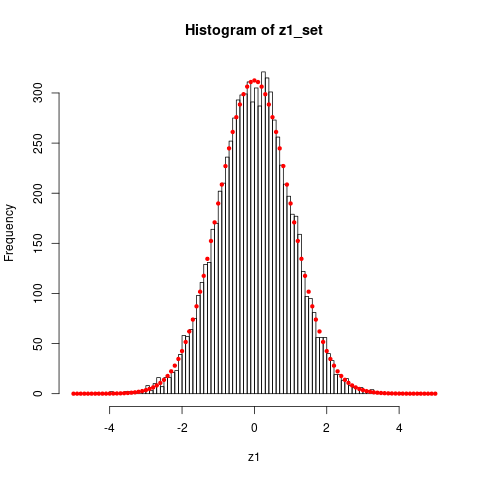
\includegraphics[height=.5\paperheight6]{ex11.png}
            \caption{histogram of z1 and gauss-fit}
        \end{figure}
        
        \begin{figure}[H]
            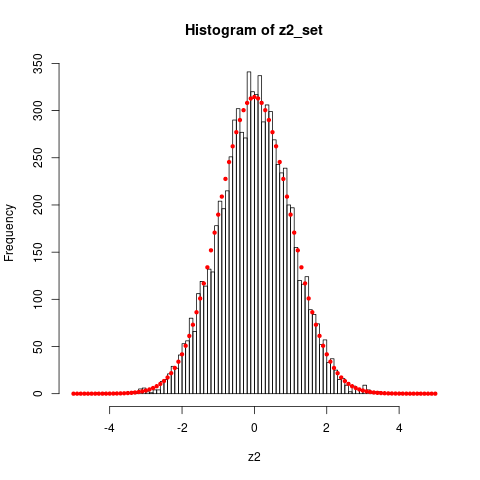
\includegraphics[height=.5\paperheight]{ex12.png}
            \caption{histogram of z2 and gauss-fit}
        \end{figure}     
    \newpage
    
    \section{Random Walk}
        We generate the mean number of steps needed for a 1D random walk as a function of the distance n
        
        
        \begin{figure}[H]
            \lstinputlisting{ex2.R}
            \caption{ex2.R}
        \end{figure}
    
        \begin{figure}[H]
            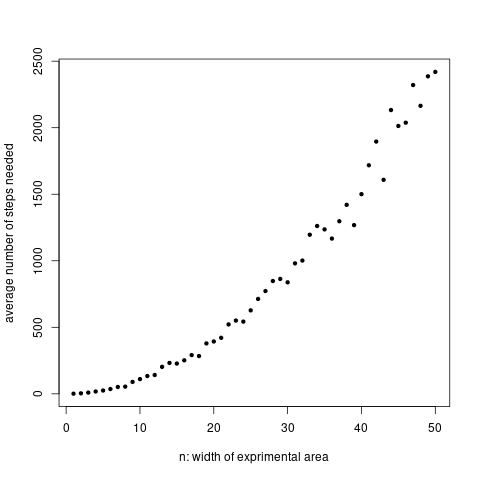
\includegraphics[height=.5\paperheight]{ex2.png}
            \caption{average number of steps taken as a function of n, in 50 tests per n}
        \end{figure}
    
        we can assume the number of steps required rises exponentially with the distance n
\end{document}
